% Section name and highlighted ToC
\renewcommand{\sectiontitle}{Partition into Triangles}
\section{\sectiontitle}
\customToC{currentsection,hideothersubsections}{}

\begin{frame}{\sectiontitle}
    \begin{itemize}
        \itemj Ejemplar genérico: Una gráfica $G=(V,E)$, con $|V|=3q$ para un entero positivo $q$.
        \item Pregunta de decisión: Hay una partición de $V$ en $q$ conjuntos disjuntos $V_1,V_2,...,V_q$ de tres vértices cada uno tal que para cada $V_i=\{v_{i[1]},v_{i[2]},v_{i[3]}\}$, las tres aristas $\{v_{i[1]},v_{i[2]}\},\{v_{i[1]},v_{i[3]}\},\{v_{i[2]},v_{i[3]}\}$ pertenezcan a $E$?
    \end{itemize}
\end{frame}

\renewcommand{\subsectiontitle}{Algoritmo no determinista}
\subsection{\subsectiontitle}

\begin{frame}{\subsectiontitle}
    \begin{itemize}
    \itemj Fase Adivinadora\\
    \begin{itemize}
        \item Sabemos que $|V| = 3q$ entonces supongamos que tenemos un dado equilibrado de $q$ lados. Para cada $v\in V$ tiramos nuestro dado, sea $n$ el número obtenido por el dado, si el subconjunto de vértices $V_n$ tiene menos de 3 vértices entonces agregamos el vértice $v$ a $V_n$, si el subconjunto de vértices $V_n$ ya tiene 3 vértices entonces buscamos el siguiente $V_m$ que tenga menos de 3 vértices y agregamos $v$ a $V_m$, si llegamos a $V_q$ y no pudimos agregar a $v$ entonces desde $V_n$ buscamos el anterior $V_l$ que tenga menos de 3 vértices y agregamos $v$ a $V_l$, esto lo hacemos hasta recorrer por completo $V$.
    \end{itemize}
    

    \item Fase Verificadora\\

    \begin{itemize}
        \item Si la cardinalidad del conjunto de vértices de la gráfica $G$ no es múltiplo de 3 ningún candidato a solución será válido, entonces devolvemos NO en dicho caso.
        
        \item Si por cada subconjunto de 3 vértices $u,v,w \in V_i$ tenemos que las aristas\\ $(u,v),(u,w),(v,w)\in E$ entonces regresamos SI en otro caso regresamos NO.
    \end{itemize}

    
    
     
    
\end{itemize}
\end{frame}

% Section name and highlighted ToC
\renewcommand{\subsectiontitle}{Teorema y Demostración}
\subsection{\subsectiontitle}
% \customToC{currentsection,hideothersubsections}{}

\begin{frame}{\subsectiontitle}
    \begin{itemize}
        \itemj Teorema: El problema partición en traingulos es NP-Completo.
        \item Demostración: Transformamos cobertura exacta por conjuntos de 3 a partición en triangulos.
        \item Para demostrar el problema usaremos la técnica de reemplazo local. Pero primero ¿qué es la cobertura exacta por conjuntos de 3?
    \end{itemize}
\end{frame}

\renewcommand{\subsectiontitle}{Cobertura exacta por conjuntos de 3 (X3C)}
\subsection{\subsectiontitle}

\begin{frame}{\subsectiontitle}
    \begin{itemize}
        \itemj Ejemplar genérico: Un conjunto $X$ con $|X|=3q$ y una colección $C$ de subconjuntos de 3 elementos de $X$.
        \item Pregunta de decisión: ¿Existe algún subconjunto $C'$ de $C$ en donde cada elemento de $X$ aparezca \textbf{exactamente una vez} en $C'$? 
        \item Ejemplo: Supongamos que tenemos $X=\{1,2,3,4,5,6\}$.\\
        Si tenemos $C=\{\{1,2,3\},\{2,3,4\},\{1,2,5\},\{2,5,6\},\{1,5,6\}\}$, entonces podríamos elegir $C'=\{\{2,3,4\},\{1,5,6\}\}$ como cobertura exacta porque cada elemento de $X$ aparece \textbf{exactamente una vez}.
    \end{itemize}
\end{frame}

\renewcommand{\subsectiontitle}{Transformación}
\subsection{\subsectiontitle}

\begin{frame}{\subsectiontitle}
    \begin{itemize}
        \itemj Sea $X$ el conjunto con $|X|=3q$ y la colección $C$ de subconjuntos de 3 elementos de $X$ un ejemplar de $X3C$, construiremos una gráfica $G=(V,E)$ con
    $|V|=3q'$ tal que la partición deseada exista para $G$ si y solo si $C$ contiene una cobertura exacta.
        \item Las unidades básicas del ejemplar de $X3C$ son los subconjuntos de 3 elementos de $C$.
        \item El reemplazo local, por cada subconjunto $c_i=\{x_i,y_i,z_i\}\in C$, crea la siguiente gráfica:
    \end{itemize}
\end{frame}
\begin{frame}{\subsectiontitle}
    \begin{figure}
    \centering
        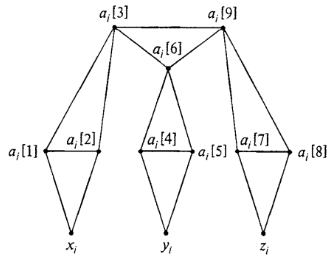
\includegraphics[width=.6\textwidth]{imgs/PIT/graficaPIT.png}
    \end{figure}
\end{frame}
\begin{frame}{\subsectiontitle}
    Así $G=(V,E)$ se define como
    \begin{align*}
        &V = X \cup \bigcup_{i=1}^{|C|} \{a_i[j]: 1\leqslant j\leqslant 9\}\\
        &E =\bigcup_{i=1}^{|C|}E_i
    \end{align*}

    Notemos que sólo los vértices que se conectan con aristas que pertenecen a más de un $E_i$ son aquellos que se encuentran en el conjunto $X$.\\

    \vspace{10pt}
    También podemos ver que $|V| = |X| + 9|C| = 3q + 9|C|$ así que $q'=q+3|C|$.
\end{frame}
\begin{frame}{Complejidad en tiempo de la transformación}
    La transformación del ejemplar de X3C al ejemplar de partición en triangulos se hace en tiempo polinomial. Tenemos que por cada subconjunto en $C$ se agregaran 12 vértices y 18 aristas a los respectivos conjuntos, lo que hace que la complejidad tenga $30|C|$ operaciones, lo que deja la complejidad en tiempo como $O(|C|)$.
\end{frame}

\begin{frame}{X3C = YES =$>$ PIT = YES}
    Si $c_1,c_2,...,c_q$, los subconjuntos de 3 elementos de $C$, están en alguna cobertura exacta para $X$, entonces la partición correspondiente $V=V_1 \cup V_2 \cup ... \cup V_q$ de $V$ está dada al tomar
    \begin{align*}
        \{a_i[1],a_i[2],x_i\},\{a_i[4],a_i[5],y_i\},\{a_i[7],a_i[8],z_i\}, \{a_i[3],a_i[6],a_i[9]\}
    \end{align*}
    de los vértices conectados por $E_i$ cuando $c_i=\{x_i,y_i,z_i\}$ está en la cobertura exacta.\\

    \vspace{10pt}
    Y tomando
    \begin{align*}
        \{a_i[1],a_i[2],a_i[3]\},\{a_i[4],a_i[5],a_i[6]\},\{a_i[7],a_i[8],a_i[9]\}
    \end{align*}
    de los vértices conectados por $E_i$ cuando $c_i=\{x_i,y_i,z_i\}$ no está en la cobertura exacta. Esto asegura que cada elemento de $X$ este incluido en exactamente un subconjunto de 3 vértices en la partición\\
\end{frame}

\begin{frame}{X3C = YES $<$= PIT = YES}
    Si $V_1\cup V_2 \cup ... \cup V_q$ es una partición en triangulos de $G$, la cobertura exacta está dada al elegir los $c_i\in C$ tal que $\{a_i[3],a_i[6],a_i[9]\}=V_j$ para alguna j, $1\leqslant j \leqslant q'$
\end{frame}

\renewcommand{\subsectiontitle}{Ejemplo de transformación}
\subsection{\subsectiontitle}

\begin{frame}{\subsectiontitle}
    Supongamos que tenemos un ejemplar de X3C con un conjunto $X=\{1,2,3,4,5,6\}$ y una colección $C=\{\{1,4,6\},\{2,4,6\},\{2,3,5\}\}$, entonces nuestro ejemplar de partición en triángulos nos quedaría como
\end{frame}
\begin{frame}
    \begin{figure}
    \centering
        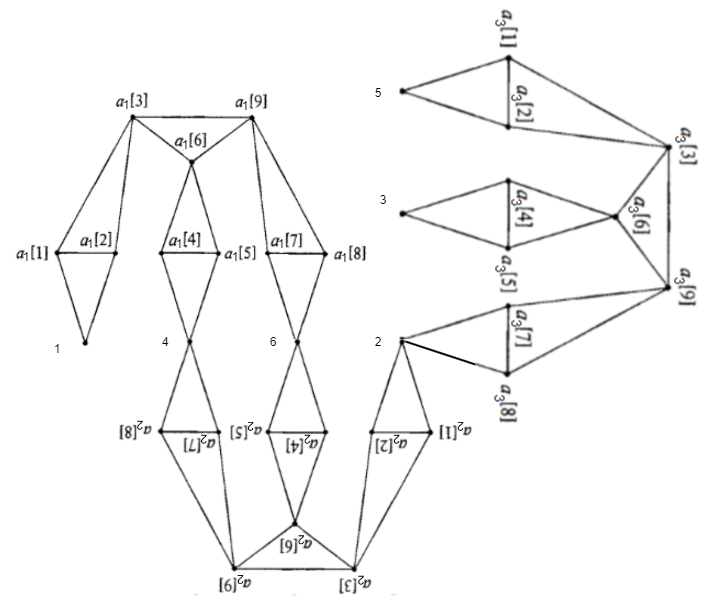
\includegraphics[width=.7\textwidth]{imgs/PIT/EjemploPIT.png}
    \end{figure}
\end{frame}